% 2020 全国Ⅱ卷 文20：三棱柱 ABC-A1B1C1 与截面四边形 EB1C1F
% 来源 PDF：普通高考/2020/2020全国2文(…).pdf 第 2 页（A3 横排），印面 1124，第 20 题题干下方
% 结构：底面 ABC 为正三角形，侧面 BB1C1C 为矩形（BB1⊥BC）；M、N 为 BC、B1C1 的中点，
%       O 为 △A1B1C1 的中心，P 为 AM 上一点（AP = AM/3），截面 EB1C1F 与底面交于 EF（EF∥BC）。
% 实线：A1A、A1B1、A1C1、B1C1、C1C、CB、BA、B1B、NM、B1E，以及原页所绘的矩形对角线 BC1；
% 虚线：AC、AO、AM（含点 P）、EF、FC1、PN（原页为标出 ∠MPN 而作）。
% 投影取自原页 300 dpi 量取的顶点位置，M、N、O 按中点/重心精确算出，E、F、P 取 AM 的三等分点。
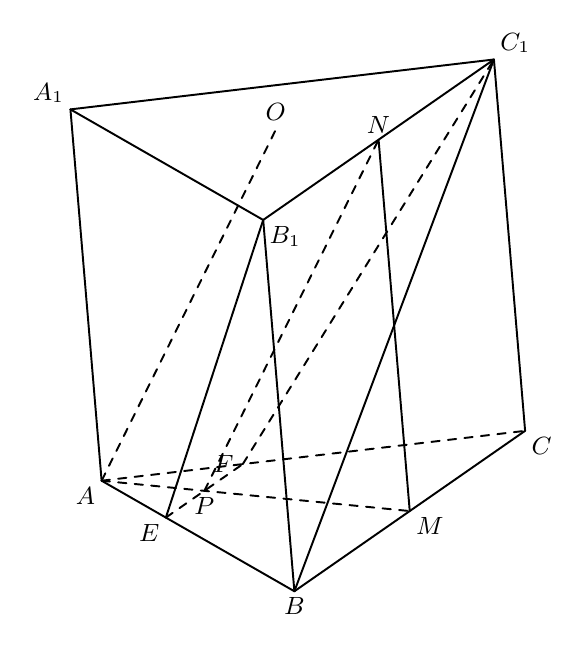
\begin{tikzpicture}[line width=0.7pt, font=\small,
  x=0.72cm, y=0.72cm, line cap=round, line join=round]

  % 顶点
  \coordinate (A1) at (0.15,9.50);
  \coordinate (B1) at (3.55,7.55);
  \coordinate (C1) at (7.62,10.38);
  \coordinate (A)  at (0.70,2.95);
  \coordinate (B)  at (4.10,1.00);
  \coordinate (C)  at (8.17,3.83);

  % 中点、重心与截面点
  \coordinate (M)  at (6.135,2.415);
  \coordinate (N)  at (5.585,8.965);
  \coordinate (O)  at (3.773,9.143);
  \coordinate (E)  at (1.833,2.300);
  \coordinate (F)  at (3.190,3.243);
  \coordinate (P)  at (2.512,2.772);

  % 可见棱
  \draw (A1) -- (A);
  \draw (A1) -- (B1);
  \draw (A1) -- (C1);
  \draw (B1) -- (C1);
  \draw (B1) -- (B);
  \draw (C1) -- (C);
  \draw (B)  -- (C);
  \draw (A)  -- (B);

  % 中位线与截面可见边
  \draw (N) -- (M);
  \draw (B1) -- (E);

  % 矩形 BB1C1C 的对角线 BC1（原页实线）
  \draw (B) -- (C1);

  % 被遮挡的棱与内部辅助线
  \draw[dashed] (A) -- (C);
  \draw[dashed] (A) -- (O);
  \draw[dashed] (A) -- (M);
  \draw[dashed] (E) -- (F);
  \draw[dashed] (F) -- (C1);
  \draw[dashed] (P) -- (N);

  % 顶点标注
  \node[above left,  inner sep=2pt] at (A1) {$A_1$};
  \node[below left,  inner sep=2pt] at (A)  {$A$};
  \node[below,       inner sep=2pt] at (B)  {$B$};
  \node[below right, inner sep=2pt] at (C)  {$C$};
  \node[above right, inner sep=2pt] at (C1) {$C_1$};
  \node[below right, inner sep=2pt] at (B1) {$B_1$};
  \node[above,       inner sep=2pt] at (N)  {$N$};
  \node[above,       inner sep=3pt] at (O)  {$O$};
  \node[below right, inner sep=2pt] at (M)  {$M$};
  \node[below left,  inner sep=2pt] at (E)  {$E$};
  \node[left,        inner sep=3pt] at (F)  {$F$};
  \node[below,       inner sep=2pt] at (P)  {$P$};
\end{tikzpicture}
